\chapter{Lecture 6: ....}\label{lec:6}
\begin{center}
  {\LARGE\bfseries\color{aaublue}
    MM6 subsection Networks and Systems}\\[0.4em]
  {\large\color{accentgray}
    Topic Notes: TCP revision / basic introduction}\\[0.2em]
  {\large\bfseries Slides 1--11}\\[0.3em]
  {\small\color{accentgray}
    Hans-Peter Schwefel, Aalborg University}
\end{center}
 
\vspace{0.5em}\hrule\vspace{1em}
\section{Transport Layer Protocols}

\subsection{1. Transport Layer Goal}

“data transfer between application (processes) in end-systems”

This means:
\begin{itemize}
    \item The \textbf{network layer (IP)} moves packets between machines (host $\rightarrow$ host)
    \item The \textbf{transport layer (TCP/UDP)} moves data between programs running on those machines
\end{itemize}

So instead of just “computer A talks to computer B”, it becomes:

\begin{quote}
Chrome on your laptop talks to a web server process on a remote machine.
\end{quote}

These programs are called \textbf{processes}.

\subsection{3. Socket API}

“e.g. socket API”

A \textbf{socket} is:
\begin{itemize}
    \item the programming interface an application uses to send/receive data over TCP/UDP
\end{itemize}

Think of it as:
\begin{itemize}
    \item a “mailbox endpoint” for a process
    \item or a handle the OS gives a program to talk on the network
\end{itemize}

\subsection{4. How a Connection is Identified}

A TCP connection is uniquely identified by a \textbf{4-tuple}:

\begin{itemize}
    \item Source IP address
    \item Source port
    \item Destination IP address
    \item Destination port
\end{itemize}

Sometimes also:
\begin{itemize}
    \item Protocol (TCP vs UDP)
\end{itemize}

\subsection{What Multiplexing Really Means}

\subsubsection{Sending Side (Multiplexing)}

The transport layer:
\begin{itemize}
    \item takes data from many application processes
    \item attaches port numbers (and uses IP underneath)
    \item sends everything through the same network interface
\end{itemize}

So the system can share the network across many applications at once.

\subsubsection{Receiving Side (Demultiplexing)}

The transport layer:
\begin{itemize}
    \item looks at incoming packets
    \item checks destination port (and IP, etc.)
    \item delivers each packet to the correct application
\end{itemize}

That is demultiplexing.

\subsection{Example Setup}

Your computer (client):
\begin{itemize}
    \item IP: 192.168.1.10
    \item Applications: Chrome, Spotify
\end{itemize}

Server:
\begin{itemize}
    \item IP: 93.184.216.34
\end{itemize}

\subsubsection{Sending Side (Multiplexing)}

Chrome connection:
\begin{itemize}
    \item Src IP: 192.168.1.10
    \item Src Port: 51512
    \item Dst IP: 93.184.216.34
    \item Dst Port: 443
\end{itemize}

Spotify connection:
\begin{itemize}
    \item Src IP: 192.168.1.10
    \item Src Port: 51513
    \item Dst IP: 151.101.2.0
    \item Dst Port: 443
\end{itemize}

\subsubsection{What the OS is doing}

\begin{verbatim}
Chrome data   ─┐
Spotify data  ─┼──> Transport layer (TCP)
Game data     ─┘
\end{verbatim}

It turns them into separate TCP segments, each tagged with:
\begin{itemize}
    \item different source ports
    \item shared network interface
\end{itemize}

Then sends them over WiFi/Ethernet.

\textbf{That’s multiplexing:}

\begin{quote}
many application streams $\rightarrow$ one network pipe
\end{quote}


\section{TCP: Connection Establishment (3-way handshake)}
\begin{figure}[H]
    \centering
    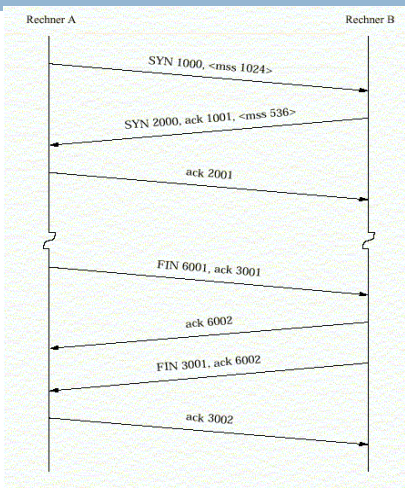
\includegraphics[width=0.6\linewidth]{figures/Lecture6/handshake.png}
    \label{fig:placeholder}
\end{figure}
TCP is a \textbf{connection-oriented protocol}, meaning both sides must agree before sending real data.

This is done using the \textbf{3-way handshake}.

\subsection{Step 1: SYN (Client $\rightarrow$ Server)}

Client sends:

\begin{quote}
“I want to start a connection”
\end{quote}

This is a \textbf{SYN packet} (synchronization request).

It includes:
\begin{itemize}
    \item A starting sequence number (e.g. \texttt{Seq = x})
\end{itemize}

\subsubsection*{Why sequence numbers matter}

TCP numbers bytes so both sides can:
\begin{itemize}
    \item track received data
    \item reorder packets if needed
    \item detect missing data
\end{itemize}

So the client is effectively saying:
\begin{quote}
“Start numbering my data from x”
\end{quote}

\subsection{Step 2: SYN-ACK (Server $\rightarrow$ Client)}

Server responds:

\begin{quote}
“I received your request and I agree”
\end{quote}

It sends:
\begin{itemize}
    \item SYN (server also starts its own connection)
    \item ACK (acknowledges client’s SYN)
\end{itemize}

It includes:
\begin{itemize}
    \item Server initial sequence number (e.g. \texttt{Seq = y})
    \item Acknowledgement number: \texttt{Ack = x + 1}
\end{itemize}

Meaning:
\begin{quote}
“I got your SYN (x), and I’m ready too”
\end{quote}

Now both sides:
\begin{itemize}
    \item agreed to communicate
    \item exchanged initial sequence numbers
\end{itemize}

\subsection{Step 3: ACK (Client $\rightarrow$ Server)}

Client replies:

\begin{quote}
“I received your response”
\end{quote}

It sends:
\begin{itemize}
    \item ACK only
    \item \texttt{Ack = y + 1}
\end{itemize}

Meaning:
\begin{quote}
“Connection is established”
\end{quote}

\section{Maximum Segment Size (MSS)}

During the handshake, both sides agree on:

\begin{quote}
“How large can each TCP segment be?”
\end{quote}

This is the \textbf{Maximum Segment Size (MSS)}.

\subsection*{Why it matters}

\begin{itemize}
    \item avoids fragmentation
    \item improves efficiency
\end{itemize}

So they negotiate something like:
\begin{quote}
“I can handle $\sim$1460 bytes of TCP payload”
\end{quote}

\section{TCP: Connection Termination}

TCP closes connections in a controlled way because it is \textbf{full-duplex} (each direction is independent).

\subsection{Step 1: FIN (one side $\rightarrow$ other side)}

A side sends:

\begin{quote}
“I am done sending data”
\end{quote}

This is a \textbf{FIN flag}.

\begin{itemize}
    \item Only closes one direction of communication
    \item The other side can still send data
\end{itemize}

So:
\begin{itemize}
    \item A $\rightarrow$ B stops sending
    \item B $\rightarrow$ A can still continue
\end{itemize}

\subsection{Step 2: ACK (other side)}

The receiver replies:

\begin{quote}
“I acknowledge your FIN”
\end{quote}

Now one direction is closed.

Later, the other side also sends:
\begin{itemize}
    \item FIN
    \item ACK
\end{itemize}

So full closure requires:
\begin{quote}
Two FIN exchanges (one per direction)
\end{quote}

\section{RST (Reset)}

Sometimes TCP does not close gracefully.

Instead it sends a \textbf{RST (reset)}.

Meaning:
\begin{quote}
“Drop this connection immediately”
\end{quote}

Used when:
\begin{itemize}
    \item port is closed
    \item application crashed
    \item invalid connection attempt
    \item forced abort
\end{itemize}
\clearpage
\section{When does the TCP handshake happen?}

The \textbf{3-way handshake} happens only when a TCP connection is created, for example:

\begin{itemize}
    \item You open a website (browser $\rightarrow$ server)
    \item You connect to a game server
    \item You start a file download
\end{itemize}

So:

\begin{quote}
\textbf{One connection = one handshake}
\end{quote}

After that, you can send many packets without repeating SYN / SYN-ACK / ACK.

\section{What happens after the handshake?}

Once the connection is established:

\begin{itemize}
    \item packet 1
    \item packet 2
    \item packet 3
\end{itemize}

No more handshake is needed.

\section{Sequence numbers}

Sequence numbers continue after the handshake.

\subsection{Step 1: handshake}

\begin{itemize}
    \item Client SYN: \texttt{Seq = 1000}
    \item Server SYN-ACK: \texttt{Seq = 5000, Ack = 1001}
    \item Client ACK: \texttt{Ack = 5001}
\end{itemize}

Now the connection is established.

\subsection{Step 2: data transfer}

\begin{itemize}
    \item Packet 1: \texttt{Seq = 1001}, Data = "Hello"
    \item Packet 2: \texttt{Seq = 1006}, Data = "World"
\end{itemize}

Notice that sequence numbers increase based on \textbf{bytes sent, not packets}.

If "Hello" is 5 bytes:

\begin{quote}
Next \texttt{Seq = 1001 + 5 = 1006}
\end{quote}

\section{Key idea}

TCP sequence numbers are:

\begin{quote}
a continuous byte counter for the whole connection
\end{quote}

NOT:

\begin{quote}
a packet counter
\end{quote}

\section{Do we ever handshake again?}

Only if:

\subsection{1. New connection is created}
e.g. a new tab opens a new TCP connection

\subsection{2. Connection breaks}
\begin{itemize}
    \item timeout
    \item network failure
    \item reset (RST)
\end{itemize}

\subsection{3. Connection is closed and reopened}
e.g. server or client restarts communication


\begin{notebox}
\textbf{Summary of handshake:}
The TCP handshake happens \textbf{once per connection}, and after that all data flows using a continuous byte-based sequence number space until the connection is closed.
\end{notebox}



\section{TCP Flow Control vs Congestion Control}

TCP controls how fast it sends data, but for two different reasons.

\section{1. Flow Control (Receiver Protection)}

\subsection*{Goal}

\begin{quote}
Do not overwhelm the receiver
\end{quote}

The receiver has a buffer (memory). If the sender is too fast:
\begin{itemize}
    \item buffer fills up
    \item data is lost
\end{itemize}

\subsection*{How TCP handles it}

The receiver tells the sender:

\begin{quote}
“I can only handle X bytes more”
\end{quote}

This is called:
\begin{itemize}
    \item Receiver Window (\texttt{rwnd})
    \item Advertised Window
\end{itemize}

\subsection*{Intuition}

Think:
\begin{itemize}
    \item receiver = slow cashier
    \item sender = customer giving items
\end{itemize}

Cashier says:

\begin{quote}
“I can only hold 10 items at a time”
\end{quote}

So the sender must slow down.

\section{2. Congestion Control (Network Protection)}

\subsection*{Goal}

\begin{quote}
Do not overload the network itself
\end{quote}

Even if the receiver is fast, the network (routers) can become overloaded.

Problems:
\begin{itemize}
    \item router buffers fill up
    \item packets are dropped
    \item delays increase
\end{itemize}

\subsection*{Key Idea}

TCP tries to:

\begin{quote}
find the maximum safe sending rate without causing congestion
\end{quote}

\section{Sliding Window}

TCP limits how much data can be ``in flight''
(sent but not yet acknowledged):

\begin{quote}
Send Window = $\min(\texttt{rwnd}, \texttt{cwnd})$
\end{quote}

Where:
\begin{itemize}
    \item \texttt{rwnd} = receiver limit
    \item \texttt{cwnd} = network limit (congestion window)
\end{itemize}

Meaning:

\begin{quote}
You can only send as fast as BOTH allow
\end{quote}

\section{Congestion Window (\texttt{cwnd})}

The congestion window is TCP's ``guess'' of network capacity.

It:
\begin{itemize}
    \item starts small
    \item increases over time
    \item decreases when congestion happens
\end{itemize}

This is called:

\begin{quote}
``probing for bandwidth''
\end{quote}
\begin{figure}[H]
    \centering
    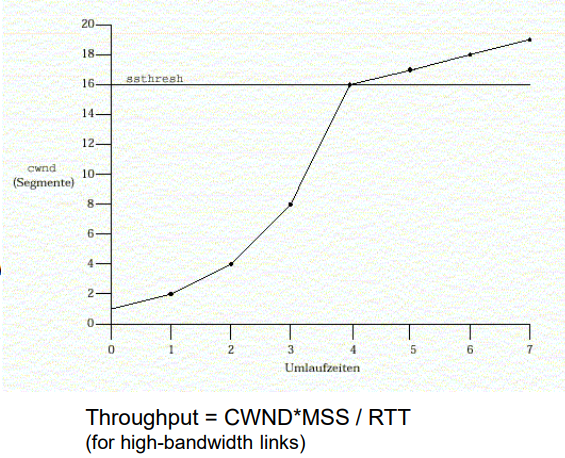
\includegraphics[width=0.7\linewidth]{figures/Lecture6/CWMD.png}
    \label{fig:placeholder}
\end{figure}

\section{Slow Start}

At the beginning:

\begin{quote}
\texttt{cwnd = 1} segment
\end{quote}

Then:

\begin{quote}
Every ACK (in each RTT ) increases \texttt{cwnd}
\end{quote}

So growth is exponential at first.

Example:

\begin{verbatim}
RTT 1: cwnd = 1
RTT 2: cwnd = 2
RTT 3: cwnd = 4
RTT 4: cwnd = 8
\end{verbatim}

\section{Slow-Start Threshold (\texttt{ssthresh})}

\subsection*{How is \texttt{ssthresh} set initially?}

At the beginning:
\begin{itemize}
    \item TCP does not know the network capacity
    \item so \texttt{ssthresh} is usually set to a large default value
\end{itemize}

Think:

\begin{quote}
“Assume the network is large until proven otherwise”
\end{quote}

So initially:
\begin{itemize}
    \item \texttt{cwnd = 1}
    \item \texttt{ssthresh =} very large value
\end{itemize}

\subsection*{When does \texttt{ssthresh} change?}

Only when TCP detects congestion.

Congestion is detected through:
\begin{itemize}
    \item timeout
    \item triple duplicate ACKs
\end{itemize}

Both indicate:

\begin{quote}
“We pushed too hard”
\end{quote}

Then TCP sets:

\begin{quote}
\texttt{ssthresh = cwnd / 2}
\end{quote}

Meaning:

\begin{quote}
“The safe sending rate is about half of what we just tried”
\end{quote}

So:
\begin{itemize}
    \item \texttt{ssthresh} is learned dynamically
    \item it is not fixed
    \item it updates whenever congestion occurs
\end{itemize}

\section{Timeout vs Triple Duplicate ACK}

\subsection{1. Timeout}

Meaning:
\begin{itemize}
    \item packet was sent
    \item ACK never arrived
    \item sender is unsure what happened
\end{itemize}

Possible causes:
\begin{itemize}
    \item packet loss
    \item severe congestion
    \item network delay collapse
\end{itemize}

TCP reaction:
\begin{itemize}
    \item \texttt{ssthresh = cwnd / 2}
    \item \texttt{cwnd = 1}
\end{itemize}

This restarts slow start.

Intuition:

\begin{quote}
“I lost visibility of the network subsection start over carefully”
\end{quote}

\subsection{2. Triple Duplicate ACKs}

Meaning:

\begin{quote}
“I am still receiving packets, but one specific packet is missing”
\end{quote}

Receiver repeatedly ACKs the same byte number.

Example:

\begin{verbatim}
Packet 1 OK  -> ACK 2
Packet 2 LOST
Packet 3     -> ACK 2
Packet 4     -> ACK 2
Packet 5     -> ACK 2
\end{verbatim}
\textbf{Acknowledge that ACK (2) is the seq nr increased of 1 by the packet 1, so we still just ACK the same packet 4 times 3 (duplicates)}

After 3 duplicate ACKs, sender realizes:

\begin{quote}
“Packet 2 is missing, but the network is still flowing”
\end{quote}

Key idea:
\begin{quote}
The network is not fully broken
\end{quote}

TCP reaction:
\begin{itemize}
    \item \texttt{ssthresh = cwnd / 2}
    \item \texttt{cwnd \approx ssthresh}
    \item immediately retransmit missing packet
\end{itemize}

This is not a full reset.

\section{Fast Retransmit}

Normally TCP waits for a timeout before retransmitting.

With 3 duplicate ACKs, TCP already knows which packet is missing.

So it:
\begin{itemize}
    \item retransmits immediately
    \item does not wait for timeout
\end{itemize}

\begin{quote}
Fast Retransmit = resend lost packet immediately after 3 duplicate ACKs
\end{quote}
\clearpage
\section{Impact of Slow Start}

\subsection*{Larger connection volume $\rightarrow$ higher average throughput}

If a TCP connection only transfers a small amount of data, throughput is often poor.

\subsection*{Why?}

Because TCP starts cautiously using \textbf{slow start}:

\begin{verbatim}
cwnd = 1
then 2
then 4
then 8
...
\end{verbatim}

TCP needs time to ramp up its sending rate.

\subsection{Small Transfer Example}

Suppose:
\begin{itemize}
    \item A webpage only needs a few packets
\end{itemize}

The transfer may finish before TCP fully ramps up its congestion window.

So:
\begin{itemize}
    \item Sender never reaches high sending rates
    \item Average throughput stays low
\end{itemize}

\subsection{Large Transfer Example}

Suppose:
\begin{itemize}
    \item Downloading a large file
\end{itemize}

Now TCP has enough time to:
\begin{itemize}
    \item increase \texttt{cwnd}
    \item send more data simultaneously
    \item approach network capacity
\end{itemize}

So average throughput becomes much higher.

\section{Throughput Upper Limits}

Even after slow start finishes, TCP throughput still has limits.

The maximum throughput is bounded by:

\[
\text{Throughput} \leq \min \left(
\text{Layer-2 throughput},
\frac{\text{Window Size}}{\text{RTT}}
\right)
\]

\subsection{1. Layer-2 Throughput Limit}

This is the physical network limit.

Examples:
\begin{itemize}
    \item WiFi speed
    \item Ethernet speed
    \item Cellular link speed
\end{itemize}

TCP cannot exceed the actual link capacity.

\subsection{2. Window Size / RTT Limit}

\[
\text{Throughput} \leq \frac{\text{Window Size}}{\text{RTT}}
\]

Where:
\begin{itemize}
    \item Window Size = amount of unacknowledged data allowed ``in flight''
    \item RTT = Round Trip Time (time for ACKs to return)
\end{itemize}

\subsection*{Intuition}

Suppose:
\begin{itemize}
    \item Window Size = 10 MB
    \item RTT = 1 second
\end{itemize}

Then sender can only send:
\begin{itemize}
    \item 10 MB every second
\end{itemize}

So maximum throughput becomes:
\begin{itemize}
    \item 10 MB/s
\end{itemize}

\subsection{Why RTT Matters}

The slide mentions:

\begin{quote}
RTT $\approx$ 1.2 seconds
\end{quote}

This is very large.

This means:
\begin{itemize}
    \item ACKs return slowly
    \item \texttt{cwnd} grows slowly
    \item sender waits longer between growth cycles
\end{itemize}

So slow start becomes much less efficient.

\begin{notebox}
\textbf{Core Takeaway}

\begin{itemize}
    \item Short TCP connections often perform poorly because slow start never fully ramps up
    \item Long connections perform better because TCP has time to increase \texttt{cwnd}
    \item TCP throughput is fundamentally limited by:
    \begin{itemize}
        \item physical link capacity
        \item window size and RTT
    \end{itemize}
\end{itemize}
\end{notebox}
\begin{figure}[H]
    \centering
    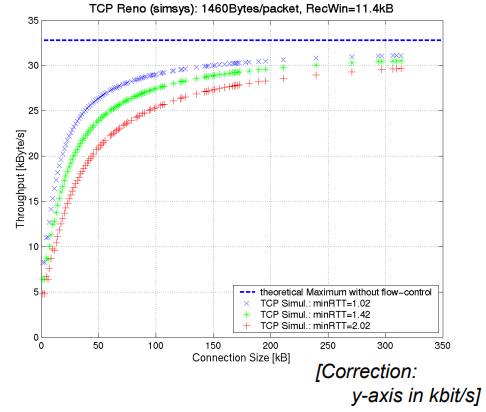
\includegraphics[width=0.75\linewidth]{figures/Lecture6/RTTeffectonTP.png}
    \label{fig:placeholder}
\end{figure}

\section{Illustration of flow control
mechanism}
\begin{figure}[H]
    \centering
    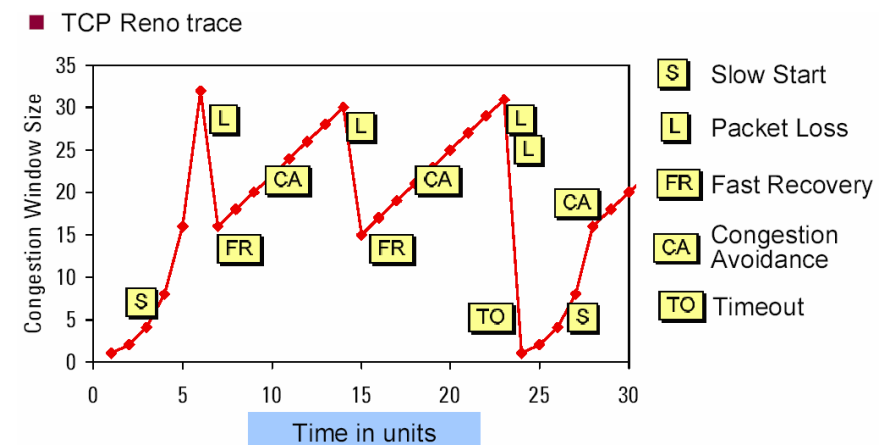
\includegraphics[width=0.9\linewidth]{figures/Lecture6/CWMDexample.png}
    \label{fig:placeholder}
\end{figure}
\section{TCP Data + ACK Behavior Options}

After the handshake, each TCP segment can behave in different ways depending on whether data and acknowledgements need to be sent.

\subsection{1. Data Only (no ACK piggyback)}

Sender sends:
\begin{itemize}
    \item \texttt{Seq = ...}
    \item \texttt{Data = ...}
\end{itemize}

Receiver responds later with:
\begin{itemize}
    \item \texttt{ACK = ...}
\end{itemize}

\textbf{Used when:}
\begin{itemize}
    \item It only needs to acknowledge received data
    \item No outgoing data is available
\end{itemize}


\subsection{2. Data + ACK (Piggybacking)}

Receiver sends:
\begin{itemize}
    \item \texttt{Seq = ...}
    \item \texttt{Data = ...}
    \item \texttt{ACK = ...}
\end{itemize}

\textbf{Used when:}
\begin{itemize}
    \item It is sending data anyway
    \item It also wants to acknowledge received data
\end{itemize}

\section{Piggybacking Idea (Optimization)}

TCP may wait a short time before sending an ACK-only packet in order to:

\begin{quote}
combine ACK + outgoing data into a single segment
\end{quote}

This reduces overhead and improves efficiency.

\subsection{Example}

\subsubsection{Client $\rightarrow$ Server}

\begin{verbatim}
Seq = 1001
Data = "Hello"
\end{verbatim}

\subsection{Server $\rightarrow$ Client (Data + ACK)}

\begin{verbatim}
Seq = 5001
Data = "Hi"
Ack = 1006
\end{verbatim}

Meaning:
\begin{itemize}
    \item \texttt{ACK = 1006} $\rightarrow$ received everything up to byte 1005
    \item \texttt{Seq = 5001} $\rightarrow$ server data starts at 5001
\end{itemize}

\begin{notebox}
\textbf{Key takeaways:}
TCP segments can carry:
\begin{itemize}
    \item only data
    \item only ACK
    \item or both together (piggybacking for efficiency)
\end{itemize}
\end{notebox}
\clearpage
\begin{center}
  {\LARGE\bfseries\color{aaublue}
    MM6 subsection Networks and Systems}\\[0.4em]
  {\large\color{accentgray}
    Topic Notes: TCP Performance: Simulation and Measurements}\\[0.2em]
  {\large\bfseries Slides 13--20}\\[0.3em]
  {\small\color{accentgray}
    Hans-Peter Schwefel, Aalborg University}
\end{center}

\section{TCP Performance Parameters (Selection)}

\section{1. TCP Segment-based Metrics (Smallest Level)}

This looks at individual packets (segments).

\subsection*{What we measure}
\begin{itemize}
    \item Number of retransmissions
    \item Number of timeout events
    \item RTT (Round Trip Time)
\end{itemize}

\subsection*{What RTT includes}

RTT is not just travel time. It includes:

\begin{itemize}
    \item Transmission delay (sending bits onto the link)
    \item Propagation delay (travel time through the network)
    \item Queueing delay (waiting in routers)
    \item Retransmission delay (if a packet was lost)
    \item ACK delay (receiver may delay acknowledgements)
\end{itemize}

\subsection*{Intuition}

This level asks:

\begin{quote}
How healthy is each packet delivery?
\end{quote}

So we check:
\begin{itemize}
    \item Is the network fast?
    \item Is it congested?
    \item Are packets getting lost?
\end{itemize}

\section{2. Connection-based Metrics (Whole Flow)}

Now we zoom out and look at the entire TCP session.

\subsection*{What we measure}
\begin{itemize}
    \item Total transfer time (e.g., file download time)
    \item Average throughput / goodput
    \item Probability of successful transfer
\end{itemize}

\section{3. Fairness (Between Connections)}

Now we zoom out even more:

\begin{quote}
How fairly do multiple TCP connections share the network?
\end{quote}

\subsection*{Bottleneck scenario}

If $N$ TCP flows share one bottleneck link, then ideal fairness is:

\[
\frac{1}{N}
\]

Each flow should get an equal share of the capacity.

\subsection*{Intuition}

If 10 users share a link:
\begin{itemize}
    \item each should get approximately 10\% of the bandwidth
\end{itemize}

\subsection*{Reality (important insight)}

TCP tries to be fair, but fairness depends on:
\begin{itemize}
    \item RTT differences
    \item congestion control behavior
    \item network topology
\end{itemize}

So fairness is not perfect.

\subsection*{Max-min fairness (multi-hop case)}

In complex networks:

\begin{quote}
Increase the smallest flows first, without hurting others unnecessarily
\end{quote}

Meaning:
\begin{itemize}
    \item flows with least bandwidth get priority
    \item no flow is reduced unless necessary to maintain fairness
\end{itemize}
\clearpage

\section{Simulation Model: Multiplexed ON/OFF Traffic}
\begin{figure}[H]
    \centering
    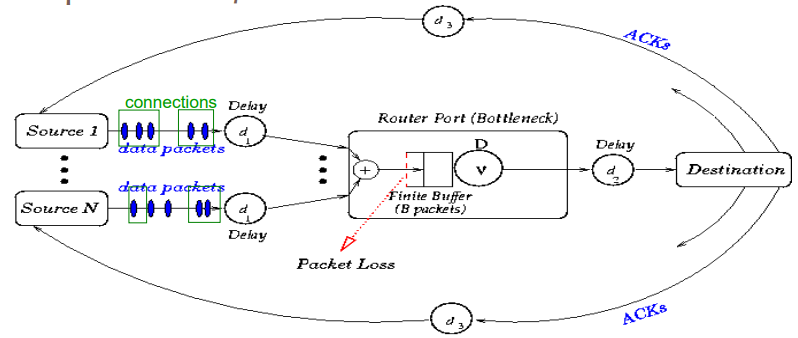
\includegraphics[width=0.9\linewidth]{figures/Lecture6/scenerioTCP.png}
    \label{fig:placeholder}
\end{figure}
\subsection*{Scenario}

We consider a scenario with $N$ ON/OFF sources.

Each source alternates between:
\begin{itemize}
    \item \textbf{ON state}: sending data
    \item \textbf{OFF state}: no transmission
\end{itemize}

This creates bursty traffic patterns that are more realistic for Internet-like behavior.

\subsection*{Multiplexed traffic}

Many ON/OFF users share the same network link.

Their packets are multiplexed, meaning:

\begin{quote}
packets from different users are mixed together on the same link
\end{quote}


\subsection*{Queueing and loss only at bottleneck router}

We assume a simplified network model where:

\begin{itemize}
    \item Only one router is congested (the bottleneck router)
    \item All queueing and packet loss occur only at this point
    \item All other parts of the network are assumed to be perfect (no loss, no delay variation)
\end{itemize}

At the bottleneck router:
\begin{itemize}
    \item packets may queue (wait in buffer)
    \item packets may be dropped (loss due to overflow)
\end{itemize}

\subsection*{Intuition}

The network is simplified to:

\begin{quote}
many users $\rightarrow$ one congested ``traffic jam'' point
\end{quote}


\subsection*{What is being measured?}

The main performance metric is:

\begin{quote}
average throughput per connection
\end{quote}

So the question is:

\begin{quote}
On average, how much bandwidth does each TCP flow receive?
\end{quote}

\begin{notebox}
\textbf{Why this model is used}
This simulation setup is used to study:
\begin{itemize}
    \item \textbf{Congestion behavior:} how TCP reacts when many flows compete for the same resource
    \item \textbf{Fairness:} whether flows share bandwidth equally or not
    \item \textbf{Throughput stability:} whether individual flows receive stable or fluctuating bandwidth
\end{itemize}
\end{notebox}
\section{Result of Simulation Model:}
\section{Correlation: Connection Size and Throughput}
\textbf{Connection Size = Total amount of data sent in one TCP connection}
\begin{figure}[H]
    \centering
    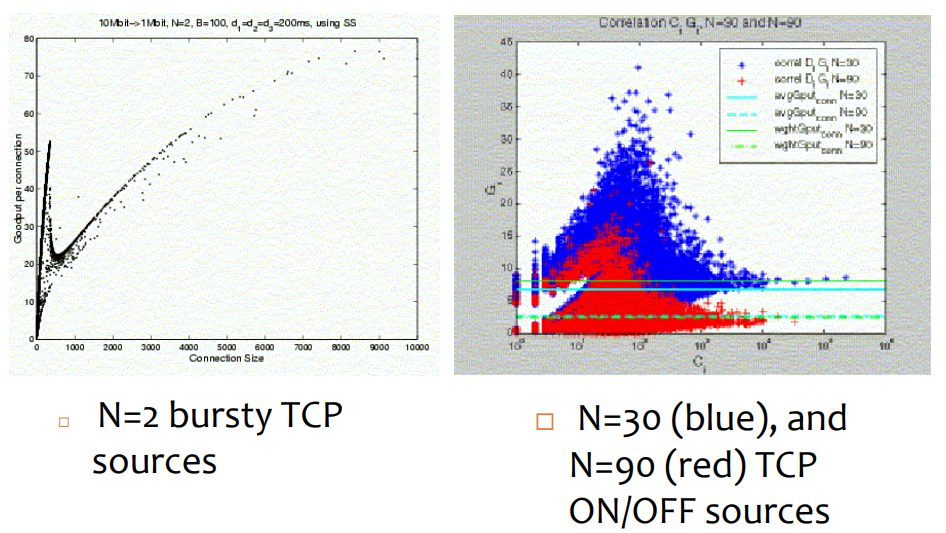
\includegraphics[width=\linewidth]{figures/Lecture6/TCPsources.png}
    \label{fig:placeholder}
\end{figure}
\subsection{Case 1: Only 2 Connections, Small Load}

If both connections send small or moderate amounts of data:

\begin{itemize}
    \item Link is not fully utilized
    \item No queue buildup at router
    \item No packet loss
\end{itemize}

\subsection*{Result}
\begin{itemize}
    \item Increasing connection size (slightly) can improve efficiency because:
    \begin{itemize}
        \item TCP ramps up (slow start effect becomes less dominant)
        \item Less relative overhead
    \end{itemize}
\end{itemize}


\subsection{Case 2: 2 Connections, Large Load (Near or Over Capacity)}

Now each connection sends a large amount of data.

Eventually:

\begin{quote}
Combined sending rate $>$ link capacity
\end{quote}

\subsection*{What happens}
\begin{itemize}
    \item Router buffer fills
    \item Queueing delay increases
    \item Packets are dropped
    \item Retransmissions occur
\end{itemize}

\subsection*{Result}
\begin{itemize}
    \item Congestion appears
    \item Goodput stops increasing
    \item Goodput may even decrease due to retransmissions
\end{itemize}

\subsection{Case 3: Many Connections}

Now many flows share one bottleneck link.

\subsection*{Effects}
\begin{itemize}
    \item More competition for buffer space
    \item More frequent congestion events
    \item More packet loss
    \item More unfairness (depending on RTT and cwnd dynamics)
\end{itemize}

\subsection*{Result}
\begin{itemize}
    \item Lower per-connection goodput
    \item Oscillations in throughput (due to cwnd variations)
    \item More retransmissions
    \item Reduced efficiency overall
\end{itemize}

\begin{notebox}
    \textbf{Key Intuition}
There are two regimes:

\subsection*{1. Underloaded Network}
\begin{itemize}
    \item No congestion
    \item Increasing connection size improves efficiency
    \item Goodput increases toward link capacity
\end{itemize}

\subsection*{2. Overloaded Network}
\begin{itemize}
    \item Bottleneck is saturated
    \item Queues and packet losses occur
    \item Goodput flattens or decreases
\end{itemize}
\end{notebox}
\section{Comparison: Models & simulation results}
\todo{skal lige havde kigge på det here}
\begin{figure}[H]
    \centering
    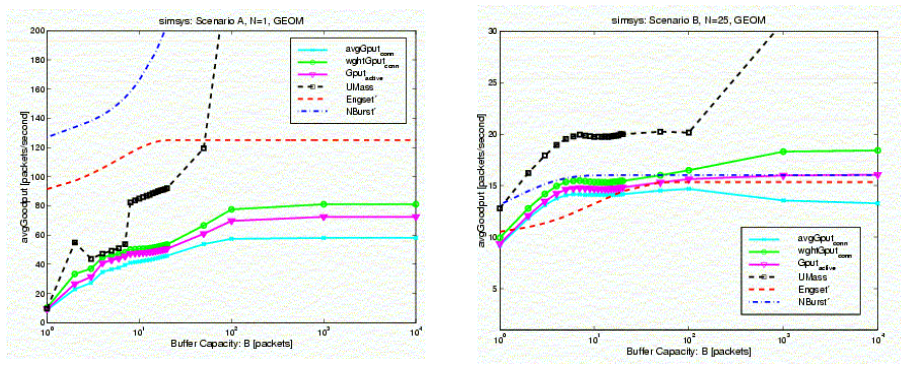
\includegraphics[width=\linewidth]{figures/Lecture6/TCPresults.png}
    \label{fig:placeholder}
\end{figure}

\section{Measurement Scenario: Static Network Setup}
\begin{figure}[H]
    \centering
    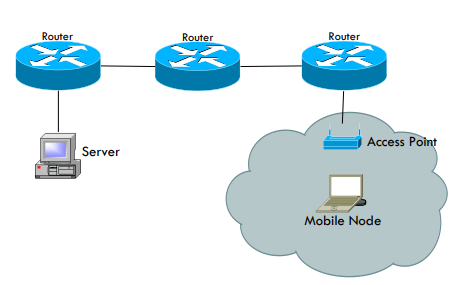
\includegraphics[width=0.5\linewidth]{figures/Lecture6/scenerioServerMobile.png}
    \label{fig:placeholder}
\end{figure}
We consider a scenario with a \textbf{single persistent TCP connection} between a mobile node and a server.

\subsection*{Meaning of ``persistent''}

\begin{itemize}
    \item The connection stays open for a long time
    \item No repeated TCP handshakes
    \item Continuous data transfer over the same connection
\end{itemize}

subsection

\subsection*{Direction of data flow}

Important detail:

\begin{quote}
Downstream only (server $\rightarrow$ mobile node)
\end{quote}

So:
\begin{itemize}
    \item Server sends data (e.g., video, file, streaming content)
    \item Mobile node mainly receives data
\end{itemize}

This simplifies the analysis by avoiding bidirectional traffic effects.

subsection

\section{Wireless Part of the Network}

Two possible wireless technologies are considered for the last hop:

subsection

\subsection{1. WLAN (802.11b)}

\begin{itemize}
    \item WiFi-based network
    \item Infrastructure mode: devices connect via an access point
\end{itemize}

\subsubsection*{DCF (Distributed Coordination Function)}

DCF is the basic medium access mechanism in WiFi.

It is based on \textbf{CSMA/CA (Carrier Sense Multiple Access with Collision Avoidance)}:

\begin{itemize}
    \item Devices first \textbf{listen} to the channel (carrier sense)
    \item If the channel is free, they transmit
    \item If the channel is busy, they wait and retry after a random backoff time
    \item This reduces the probability of collisions (since WiFi cannot easily detect collisions while transmitting)
\end{itemize}

\textbf{Intuition:}
Devices ``take turns probabilistically'' to share the wireless medium fairly.

subsection

\subsection{2. Bluetooth}

\begin{itemize}
    \item Access Point acts as a Master
    \item Devices form a Personal Area Network (PAN)
    \item More centralized control compared to WiFi
    \item Typically smaller range and simpler coordination
\end{itemize}

subsection

\section{Why include wireless technologies?}

Wireless links strongly affect performance:

\begin{itemize}
    \item Delay variation
    \item Packet loss probability
    \item Throughput fluctuations
    \item Congestion behavior at the last hop
\end{itemize}

Therefore, they model a realistic ``last hop'' access network.

subsection

\section{Performance Metric: Aggregated Throughput}

The key performance metric is the aggregated throughput:

\[
\Lambda(t) = \frac{V(t)}{t}
\]

\subsection*{Meaning of variables}

\begin{itemize}
    \item $V(t)$ = total useful (payload) data received by time $t$
    \item $t$ = elapsed time
\end{itemize}

\subsection*{Interpretation}

\begin{itemize}
    \item $\Lambda(t)$ is the average throughput up to time $t$
    \item It measures how efficiently data is delivered over time
\end{itemize}
\clearpage
\section{TCP over WLAN (802.11b)}
\begin{figure}[H]
    \centering
    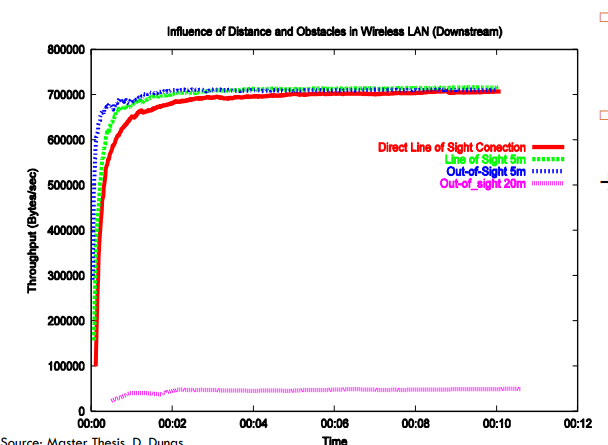
\includegraphics[width=0.8\linewidth]{figures/Lecture6/Wlanresult.png}
    \label{fig:placeholder}
\end{figure}
We study how TCP behaves when running over a WiFi (802.11b) wireless link.

\section{1. Strongly Reduced Throughput in Poor Channel Conditions}

If the WiFi channel quality is poor:

\begin{itemize}
    \item Interference increases
    \item Packets are more likely to be corrupted
    \item Transmission rates decrease (rate adaptation is triggered)
\end{itemize}

\subsection*{Result}

\begin{itemize}
    \item Less useful data is delivered per second
    \item Overall throughput decreases significantly
\end{itemize}

\subsection*{Intuition}

Even if TCP itself is functioning correctly:

\begin{quote}
the wireless link becomes the bottleneck due to physical channel limitations
\end{quote}

subsection

\section{2. No TCP Retransmissions Observed}

Interestingly, TCP retransmissions are rarely observed.

Normally:

\begin{quote}
packet loss $\rightarrow$ TCP retransmission
\end{quote}

However, in this scenario:

\begin{quote}
TCP assumes the network is reliable
\end{quote}

subsection

\section{3. WLAN Link-Layer Retransmissions}

The key reason is that WiFi (802.11) already provides reliability at the link layer.

\subsection*{Mechanism}

\begin{itemize}
    \item Each frame must be acknowledged by the receiver
    \item If no ACK is received, the frame is retransmitted at the link layer
\end{itemize}

\subsection*{Effect}

Before TCP even detects a loss:

\begin{quote}
the WLAN layer has already recovered the lost frame
\end{quote}

So TCP does not need to retransmit.

subsection

\section{4. Rate Adaptation}

WiFi also adapts the transmission rate based on channel quality:

\begin{itemize}
    \item Good channel $\rightarrow$ higher bitrate (more efficient modulation)
    \item Bad channel $\rightarrow$ lower bitrate (more robust transmission)
\end{itemize}

\subsection*{Goal}

\begin{quote}
Reduce packet loss by adapting the physical transmission speed to channel conditions
\end{quote}

subsection

\begin{notebox}
    \textbf{Overall Insight}
\begin{itemize}
    \item TCP sees a mostly loss-free channel
    \item Reliability is handled by the WLAN link layer
    \item Performance degradation is mainly due to reduced physical transmission rate, not TCP congestion control
\end{itemize}
\end{notebox}

\clearpage
\section{TCP over Bluetooth -- Main Observation}
\begin{figure}[H]
    \centering
    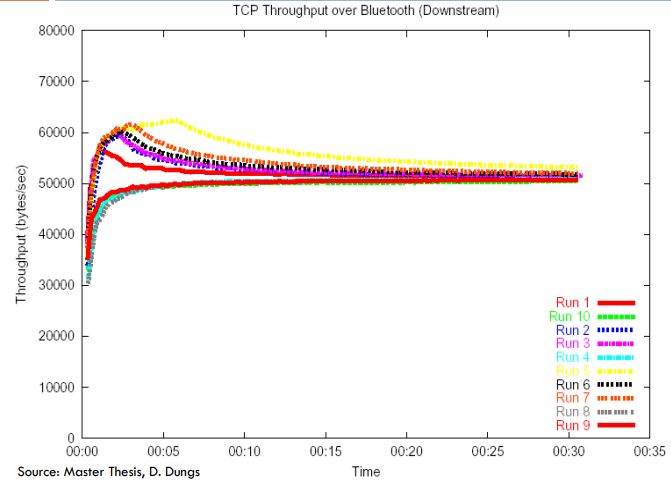
\includegraphics[width=0.8\linewidth]{figures/Lecture6/BluetoothResults.png}
    \label{fig:placeholder}
\end{figure}
\subsection*{Long-term throughput below maximum}

Even after a long time, TCP does not reach the theoretical maximum throughput.

\begin{itemize}
    \item Performance remains capped below the maximum achievable rate
    \item This limitation persists over time
\end{itemize}


\subsection*{Why no TCP retransmissions?}

As in WLAN scenarios, TCP retransmissions are not observed.

\begin{quote}
Bluetooth already handles reliability below the TCP layer
\end{quote}


\subsection*{1. Link-layer retransmissions (Bluetooth)}

Bluetooth provides reliability at the link layer:

\begin{itemize}
    \item Each frame is acknowledged (ACK)
    \item If an ACK is not received, the frame is retransmitted at the link layer
    \item Retransmissions happen locally before TCP is aware of any loss
\end{itemize}

\subsection*{Effect}

\begin{quote}
Packet losses are hidden from TCP
\end{quote}

Therefore:
\begin{itemize}
    \item TCP does not trigger retransmissions
    \item TCP assumes a relatively reliable channel
\end{itemize}


\subsection*{2. Scheduling effects (key difference in Bluetooth)}

Unlike WiFi (which uses CSMA/CA), Bluetooth uses a \textbf{master-controlled scheduling system}.

\subsubsection*{Structure}

\begin{itemize}
    \item One device acts as the \textbf{Master}
    \item Other devices are \textbf{Slaves}
    \item The master controls when each device is allowed to transmit
\end{itemize}

\subsubsection*{Implications}

\begin{itemize}
    \item Access to the medium is centrally controlled (not contention-based)
    \item Timing is deterministic and slot-based
    \item Performance limitations arise from scheduling rather than collisions
\end{itemize}

\begin{figure}[H]
    \centering
    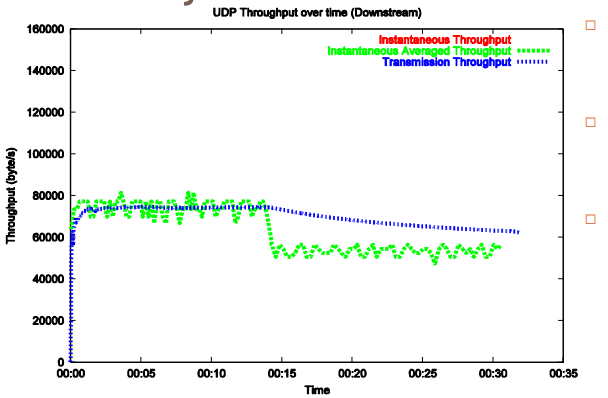
\includegraphics[width=0.8\linewidth]{figures/Lecture6/BluetoothInstantous.png}
    \label{fig:placeholder}
\end{figure}

\subsection*{3. Throughput drop after approximately 15 seconds}

The measurements show a throughput decrease of about 33\% after some time.

\subsection*{Possible explanations}

\subsubsection*{(1) Bluetooth packet scheduler effects}

\begin{itemize}
    \item Scheduling may become less efficient over time
    \item Polling or time-slot patterns may underutilize the channel
\end{itemize}

\subsubsection*{(2) Link symmetry constraints}

Bluetooth often assumes symmetric communication patterns and fixed master/slave cycles.

In a primarily downstream TCP scenario:

\begin{itemize}
    \item Reverse-direction capacity is underutilized
    \item Scheduling structure is not fully efficient for unidirectional traffic
    \item Effective throughput decreases
\end{itemize}

\subsubsection*{(3) Interference (2.4 GHz band)}

Bluetooth operates in the 2.4 GHz spectrum, shared with other technologies:

\begin{itemize}
    \item WiFi devices
    \item Other wireless interferers
\end{itemize}

\begin{itemize}
    \item Interference reduces effective transmission rate
    \item Additional link-layer retransmissions occur (not visible to TCP)
\end{itemize}

\begin{notebox}
\textbf{Key Insight}

\begin{itemize}
    \item TCP sees no losses because reliability is handled below it
    \item However, throughput is still limited by scheduling, interference, and link-layer efficiency
\end{itemize}
\end{notebox}
\clearpage
\begin{center}
  {\LARGE\bfseries\color{aaublue}
    MM6 subsection Networks and Systems}\\[0.4em]
  {\large\color{accentgray}
    Topic Notes: TCP Performance Models}\\[0.2em]
  {\large\bfseries Slides 22--26}\\[0.3em]
  {\small\color{accentgray}
    Hans-Peter Schwefel, Aalborg University}
\end{center}

\section*{Core Idea: Closed Feedback Loop in TCP}

We cannot model traffic independently from network behavior. TCP congestion control still exists, but it operates inside a \textbf{closed feedback loop} where traffic and congestion continuously influence each other.

\subsubsection*{Core feedback loop (intuitive)}

We have two interacting components:

\paragraph{1. TCP changes $cwnd$}

\begin{itemize}
    \item Changes sending rate
    \item Changes how much traffic enters the network
\end{itemize}

\paragraph{2. Network reacts (congestion)}

\begin{itemize}
    \item Queueing builds up in routers
    \item Delay increases or packets are dropped
    \item Sender receives ACKs, duplicate ACKs, or timeouts
\end{itemize}

\subsubsection*{Feedback loop behavior}

\begin{itemize}
    \item $cwnd \uparrow \rightarrow$ more traffic sent $\rightarrow$ congestion $\uparrow$
    \item congestion $\uparrow \rightarrow$ loss/delay $\uparrow \rightarrow$ $cwnd \downarrow$
    \item $cwnd \downarrow \rightarrow$ less traffic $\rightarrow$ congestion $\downarrow$
    \item congestion $\downarrow \rightarrow$ network recovers $\rightarrow$ $cwnd \uparrow$
\end{itemize}

\subsubsection*{Key intuition}

TCP is not only controlling congestion.

\begin{quote}
It continuously drives congestion and reacts to it at the same time.
\end{quote}

\subsection*{Consequence}

Because of this feedback:

\begin{itemize}
    \item It is not possible to fully separate a traffic model from a network model
    \item Classical independent modeling approaches do not work well
\end{itemize}

\subsection*{Need for new models}

To analyze TCP performance, integrated or coupled models are required.


\subsection*{Approaches}
\todo{Få kigget på slide 23-26 omrking disse modeller}
\subsubsection*{1. Connection-level models}

Example: Heyman et al. (SIGMETRICS 1997)

\begin{itemize}
    \item Model TCP connections as high-level stochastic processes
    \item Focus on connection arrivals and durations
    \item Abstract away packet-level dynamics
\end{itemize}

\subsubsection*{2. Sender/receiver behavior with fixed-point iteration}

\begin{itemize}
    \item Model sender rate as a function of network conditions
    \item Model network conditions as a function of offered load
    \item Solve iteratively until a stable equilibrium (fixed point) is reached
\end{itemize}

\subsubsection*{3. Integrated models (e.g., multiplexed ON/OFF models)}

\begin{itemize}
    \item Combine traffic generation and network behavior in one model
    \item Use ON/OFF sources to represent bursty traffic
    \item Analyze performance under shared bottleneck conditions
\end{itemize}